% This file was created by matlab2tikz.
%
%The latest updates can be retrieved from
%  http://www.mathworks.com/matlabcentral/fileexchange/22022-matlab2tikz-matlab2tikz
%where you can also make suggestions and rate matlab2tikz.
%
\documentclass[tikz]{standalone}
\usepackage[T1]{fontenc}
\usepackage[utf8]{inputenc}
\usepackage{pgfplots}
\usepackage{grffile}
\pgfplotsset{compat=newest}
\usetikzlibrary{plotmarks}
\usepgfplotslibrary{patchplots}
\usepackage{amsmath}

\begin{document}
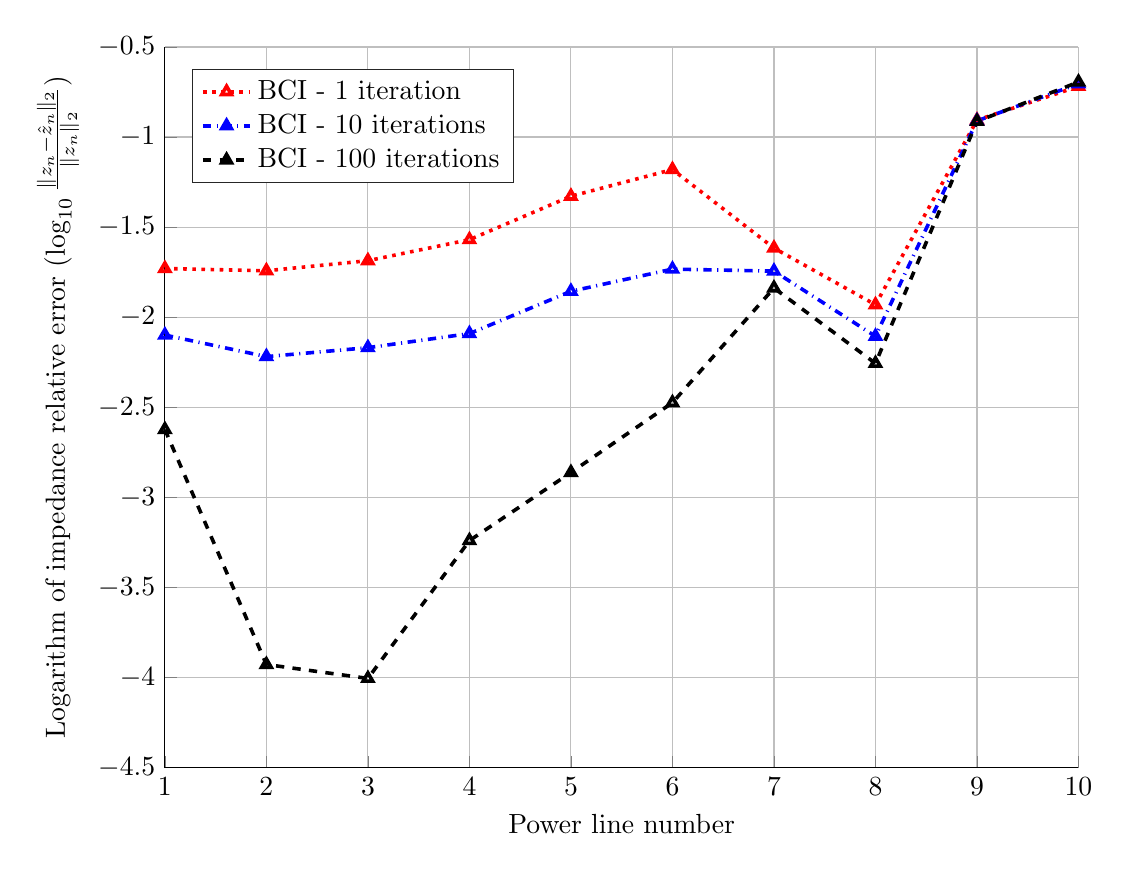
\begin{tikzpicture}

\begin{axis}[%
width=4.568in,
height=3.603in,
at={(0.766in,0.486in)},
scale only axis,
xmin=1,
xmax=10,
xlabel={Power line number},
xmajorgrids,
ymin=-4.5,
ymax=-0.5,
ylabel={Logarithm of impedance relative error ($\log_{10}\frac{\|z_n - \hat{z}_n\|_2}{\|z_n\|_2}$)},
ymajorgrids,
axis background/.style={fill=white},
axis x line*=bottom,
axis y line*=left,
legend style={at={(0.03,0.97)},anchor=north west,legend cell align=left,align=left,draw=white!15!black}
]
\addplot [color=red,dotted,line width=1.3pt,mark=triangle,mark options={solid}]
  table[row sep=crcr]{%
1	-1.72982683986341\\
2	-1.74238158217577\\
3	-1.6863928841115\\
4	-1.56978293664016\\
5	-1.32856400089715\\
6	-1.18040433328921\\
7	-1.61648897086946\\
8	-1.93096182265119\\
9	-0.906031940889947\\
10	-0.718937724561957\\
};
\addlegendentry{BCI - 1 iteration};

\addplot [color=blue,dashdotted,line width=1.3pt,mark=triangle,mark options={solid}]
  table[row sep=crcr]{%
1	-2.09919387246171\\
2	-2.21880045072973\\
3	-2.16924631102906\\
4	-2.09114366901125\\
5	-1.85626652002556\\
6	-1.73315751238561\\
7	-1.74435133973592\\
8	-2.10621158863848\\
9	-0.910383700943571\\
10	-0.70437523998247\\
};
\addlegendentry{BCI - 10 iterations};

\addplot [color=black,dashed,line width=1.3pt,mark=triangle,mark options={solid}]
  table[row sep=crcr]{%
1	-2.62355836827617\\
2	-3.92803765227028\\
3	-4.00522085976364\\
4	-3.24011793352677\\
5	-2.86206662924396\\
6	-2.47460536523476\\
7	-1.83815331409476\\
8	-2.25650922582314\\
9	-0.913263288185591\\
10	-0.694740015683183\\
};
\addlegendentry{BCI - 100 iterations};

\end{axis}
\end{tikzpicture}%
\end{document}